%\newcommand{\norm}[1]{\parallel #1\parallel}
%\newcommand{\R}{\mbox{${\Bbb R}$}}
%\newcommand{\N}{\mbox{${\mathcal N}$}}
\newcommand{\M}{\mbox{${\mathcal M}$}}
\newcommand{\A}{\mbox{${\mathcal A}$}}
\newcommand{\U}{\mbox{${\mathcal U}$}}

\subsection{Cicho\'n's diagram and cardinal characteristics}

This section will be devoted to an introduction to topic of cardinal characteristics of the continuum. Most of
these cardinal numbers are associated with some properties of the real line. They are all greater or equal
to $\omega_1$ and less or equal to $\cont$, but in general their value is not decided by the usual axioms of ZFC.
Positing that some cardinal invariant is equal to $\cont$ may be seen as a weakening of the continuum hypothesis
and in fact many constructions which work under CH may be carried out under weaker assumptions of this form.
For a beautiful exposition of the topic see \cite{Bl:2009}.

We start with the following general definition, which will be used mainly in the case that the ideal
$I$ is either the ideal of meager sets of $\R$ (denoted $\M$) or the ideal sets having \emph{Lebesgue measure zero}
(denoted by $\N$).

\begin{definition} For any ideal ${\mathcal I}$ on a set $X$ we define the following cardinal characteristics:
 \begin{eqnarray*}
  \hbox{add}({\mathcal I})  &=& min\{|{\mathcal A}|:{\mathcal A}\subseteq {\mathcal I}\ \&\ \bigcup{\mathcal A} \not\in I\}\cr
  \hbox{non}({\mathcal I}) &=& min\{|A|:A\subseteq X\ \&\ A\not\in {\mathcal I}\}\cr
  \hbox{cov}({\mathcal I})  &=& min\{|{\mathcal A}|:{\mathcal A}\subseteq {\mathcal I}\ \&\ \bigcup{\mathcal A} = \bigcup{\mathcal I}\}\cr
  \hbox{cof}({\mathcal I})  &=& min\{|{\mathcal A}|:{\mathcal A}\subseteq {\mathcal I}\ \&\ (\forall I\in{\mathcal I})(\exists A\in{\mathcal A})(I\subseteq A)\}\cr
 \end{eqnarray*}
\end{definition}
The following is a summary definition of some of the important cardinal characteristics:
\begin{definition}
 We define the following cardinals
 \begin{eqnarray*}
  {\mathfrak b} &=& min\{|\A|:\A\subseteq {}^\omega\omega\ \&\ (\forall f\in{}^\omega\omega)(\exists g\in\A)(g\not\leq^* f)\}\cr
  {\mathfrak d} &=& min\{|\A|:\A\subseteq {}^\omega\omega\ \&\ (\forall f\in{}^\omega\omega)(\exists g\in\A)(f\leq^* g)\}\cr
  {\mathfrak a} &=& min\{|\A|:\A\subseteq [\omega]^\omega\ \&\ \omega\leq|\A|\ \& (\forall B\in[\omega]^\omega)(\exists A\in\A)(|A\cap B|=\omega)\}\cr
  {\mathfrak s} &=& min\{|\A|:\A\subseteq [\omega]^\omega\ \& (\forall B\in[\omega]^\omega)(\exists A\in\A)(|A\cap B|=|(\omega\setminus A)\cap B|=\omega)\}\cr
  {\mathfrak u} &=& min\{|\U|:\U\subseteq [\omega]^\omega\ \&\ \omega\leq|\A|\ \& (\forall B\in[\omega]^\omega)(\exists A\in\U)(|A\cap B|<\omega\vee A\subseteq^* B))\}\cr
  {\mathfrak h} &=& min\{\kappa:\pw(\omega)/FIN\ \hbox{is not}\ (\kappa,\cdot,2)\hbox{-distributive}\}\cr
  {\mathfrak p} &=& min\{|\U|:\U\subseteq [\omega]^\omega\ \&\ (\forall {\mathcal V}\in[\U]^{<\omega})(|\bigcap {\mathcal V}|=\omega)\ \&\ (\forall P\in[\omega]^\omega)(\exists U\in\U)(P\not\subseteq^* U)\}\cr
  {\mathfrak t} &=& min\{|\U|:\U\subseteq [\omega]^\omega\ \&\ \U\ \hbox{is linearly ordered by}\ \subseteq^*\ \&\ (\forall P\in[\omega]^\omega)(\exists U\in\U)(P\not\subseteq^* U)\}\cr
  {\mathfrak i} &=& min\{|\A|:\A\subseteq [\omega]^\omega\ \&\ \A\ \hbox{is independent}\ \&\ (\forall \A^\prime\subseteq[\omega]^\omega)(\A^\prime\subseteq\A\rightarrow\A^\prime\ \hbox{is not independent})\}\cr
  {\mathfrak m} &=& min\{\kappa:MA_\kappa\ \hbox{fails}\}
 \end{eqnarray*}
\end{definition}

\begin{definition}A family ${\mathcal G}\subseteq[\omega]^\omega$ is \emph{groupwise dense} if it is closed under almost subsets and for any infinite partition of $\omega$ into intervals there are infinitely many intervals from the partition whose union is in ${\mathcal G}$. The \emph{groupwise density number} ${\mathfrak g}$ is now
defined to be the smallest cardinality of a set $\A$ of groupwise dense families with $\bigcap\A=\emptyset$.
\end{definition}

It turns out that it is very usefull to think of these definitions in the following way (introduced and isolated explicitly in \cite{Voj:93}, but
implicitly appearing already in \cite{Fre:84} and in an unpublished work of Miller).

\begin{definition} Suppose we are given a triple ${\mathbf A}=(A_-,A_+,R)$ consisting of a set $A_-$ of challenges a set $A_+$ of responses and
a relation $R\subseteq A_-\times A_+$. We say that $b\in A_+$ is a response to a challenge $a\in A_-$ iff $aRb$.
We define the \emph{norm} $||{\mathbf A}||=||(A_-,A_+,R)||$ of this triple to be:
\begin{displaymath}
 ||(A_-,A_+,R)||=\min\{|{\mathcal B}|:{\mathcal B}\subseteq A_+\ \&\ (\forall a\in A_-)(\exists b\in{\mathcal B})(aRb)\}.
\end{displaymath}
In other words the norm is the cardinality of the smallest set of responses which are enough to answer every challenge. We also
define the \emph{dual} ${\mathbf A}^\perp$ of ${\mathbf A}$ to be the triple $(A_+,A_,-(R^{-1}))$, where $(x,y)\in -(R^{-1})\equiv (y,x)\not\in R$.
\end{definition}

Note that most of the cardinal invariants considered so far are norms of some triple. The usefulness of this framework lies in the fact
that the notion of duality gives a precise meaning to the intuition that some of the cardinals defined (e.g. $\mathfrak b,d$) are very
intimately connected to each other.

The definition of a Tukey connection (which is a morphism between triples in the sense of category theory)

\begin{definition}[Tukey's connection] Given two ordering triples ${\mathbf A}=(A_-,A_+,R), {\mathbf B}=(B_-, B_+, Q)$ we say that ${\mathbf A}\geq_T {\mathbf B}$ if there are functions $\phi_-:B_-\to A_-$ and $\phi_+:A_+\to B_+$ which satisfy:
\begin{displaymath}
 (\forall b\in B_-, a\in A_+)(\phi_-(b)Ra\rightarrow b Q\phi_+(a))
\end{displaymath}
Following Blass we call the pair $\phi=(\phi_-,\phi_+)$ a \emph{morphism} from $\mathbf A$ to $\mathbf B$ (Vojtáš calls $\phi$ a generalized Galois-Tukey connection from $\mathbf B$ to $\mathbf A$) and we shall write $\phi:{\mathbf A}\to {\mathbf B}$. Note that if $\phi:\mathbf A\to \mathbf B$ then $\phi^\perp=(\phi_+,\phi_-)$ is
a morphism from ${\mathbf B}\perp$ to ${\mathbf A}^\perp$.
\end{definition}

It is instructive to think of $\mathbf A\geq_T \mathbf B$ as saying that meeting challenges in $\mathbf B$ is not harder then meeting challenges in $\mathbf A$,
(cf. the notion of a Borel reduction of two Borel Equivalence relations or the notion of Turing reducibility in Recursion theory).

\begin{obs} If ${\mathbf A}\leq_T{\mathbf B}$ then $\norm{{\mathbf A}}\leq_T\norm{{\mathbf B}}$.
\end{obs}

The following diagram (see \cite{Fre:84}) summarizes all that can be proved in ZFC concerning the relations between cardinal invariants defined
from the ideal of null and meager sets:

\begin{theorem}[Cincho\'n's diagram]
%\begin{displaymath}
%\begin{array}{ccccccc}
%
%\hbox{cov}({\mathcal N}) &\longrightarrow & \hbox{non}({\mathcal M}) &\longrightarrow &\hbox{cof}({\mathcal M})  &\longrightarrow & \hbox{cof}({\mathcal N})  \cr
%                         &                & \uparrow                  &                &\uparrow                  &                &                           \cr
%\uparrow                 &                & {\mathfrak b}             &\longrightarrow &{\mathfrak d}             &                &\uparrow                   \cr
%                         &                & \uparrow                  &                &\uparrow                  &                &                           \cr
%\hbox{add}({\mathcal N}) &\longrightarrow & \hbox{add}({\mathcal M})  &\longrightarrow &\hbox{cov}({\mathcal M})  &\longrightarrow & \hbox{non}({\mathcal N}) \cr
%\end{array}
%\end{displaymath}
\end{theorem}
\begin{center}
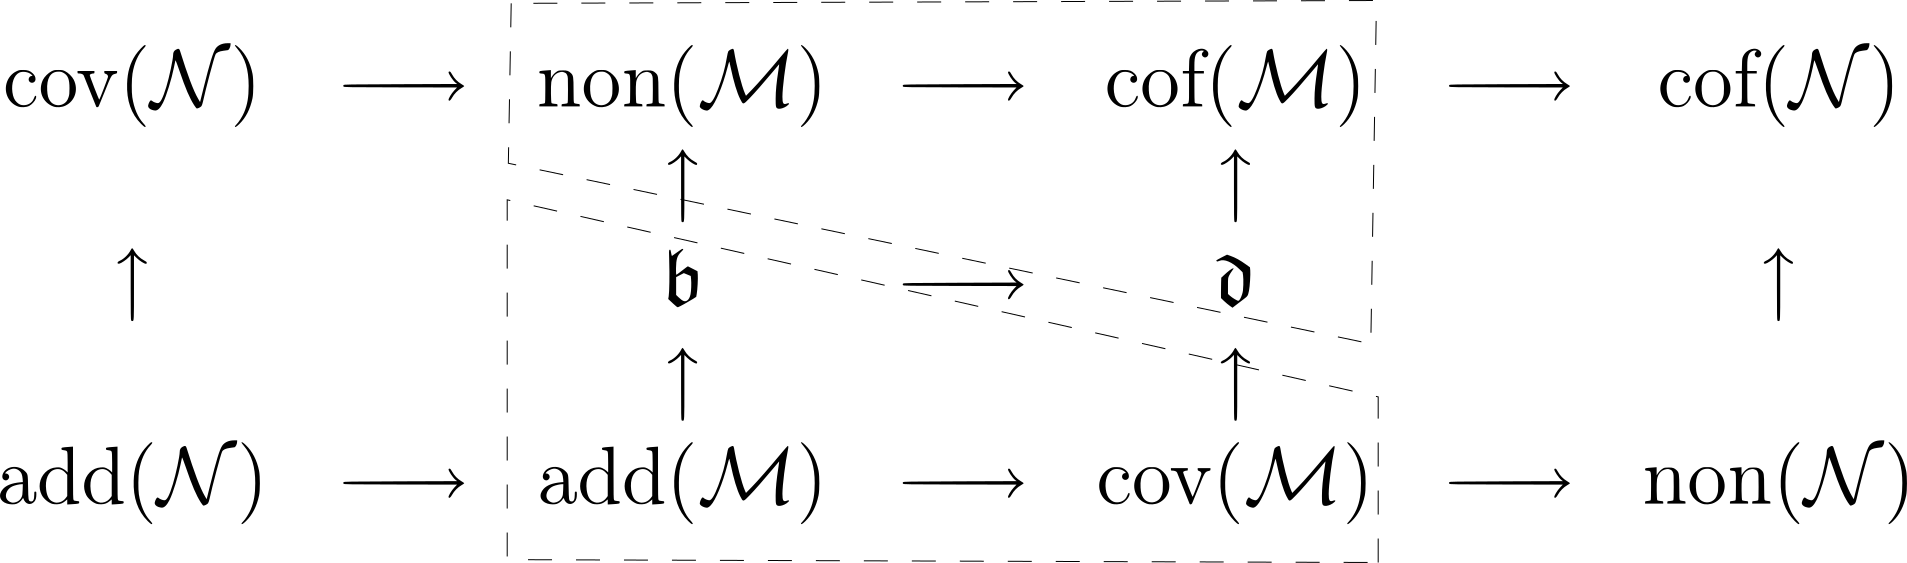
\includegraphics[height=3cm]{work_in_progress/cichon-2.pdf}
\end{center}

It is a direct consequence of the following reformulation of the cardinal invariants in terms of norms of triples:

\begin{theorem}
 \begin{displaymath}
\begin{array}{ccccccc}

(\R,\N,\in)        &\longrightarrow & (\M,\R,\not\ni)                         &\longrightarrow & (\M,\M,\subset)                    & \longrightarrow &(\N,\N,\subset)\cr
                   &                & \uparrow                                &                &\uparrow                            &                 &               \cr
\uparrow           &                & (\omega^\omega,\omega^\omega,\not\geq^*)&\longrightarrow &(\omega^\omega,\omega^\omega,\leq^*)&                 &\uparrow       \cr
                   &                & \uparrow                                &                &\uparrow                            &                 &               \cr
(\N,\N,\not\supset)&\longrightarrow & (\M,\M,\not\supset)                     &\longrightarrow &(\R,\M,\in)                         & \longrightarrow &(\N,\R,\not\ni)\cr
\end{array}
\end{displaymath}
\end{theorem}

A summary of the connections between different cardinal invariants can be seen in the following diagram. It is a fusion of
Cicho\'n's diagram with van Douwen's diagram which can be found in \cite{Bl:2009} (see also \cite{Br:2006}):

\begin{center}
\includegraphics[height=10cm]{work_in_progress/cardinal-invariants-diagram-varIII.pdf}
\end{center}

The dashed boxes indicate, respectively, that the top cardinal and bottom cardinal are the maximum and the minimum of the other
two cardinals.